\chapter{Experiments}
We now engage in our contribution to tackling the issue of automatic differential diagnosis of Mendelian diseases. In this context, we have developed a customized knowledge graph (KG) integrated with patient data, which we detail in \Cref{sec:patientKG}. Furthermore, we outline the methodology by which we have reformulated our problem as a link prediction task, demonstrating the validity of our selection of hyperbolic graph representation learning techniques (\Cref{sec:linkPredictionDiffDiagnosis}).

\section{Patient KG}\label{sec:patientKG}
In this section, we delineate the data selected for the purpose of differential diagnosis of Mendelian diseases. We proceed with an exploration of the underlying biomedical knowledge graph utilized and the patient data chosen. Additionally, we describe how these data sources have been integrated into a singular knowledge graph.

\subsection{Underlying biomedical KG}\label{sec:underlyingKG}
Initially, we considered PrimeKG \cite{chandak2023PrimeKG}, a knowledge graph aimed at precision medicine analyses that aggregates 20 high-quality resources. Unfortunately, at the time of use, we encountered significant shortcomings regarding the representation of Mendelian diseases. Drawing inspiration from the entities represented in PrimeKG, we constructed a customized knowledge graph. We have resorted to \emph{PheKnowLator} (\emph{Phenotype Knowledge Translator})~\cite{callahan2020PheKnowlator}\footnote{The Python library is accessible at \url{https://github.com/callahantiff/PheKnowLator}}, a KG framework designed for optimized construction of semantically rich, large-scale biomedical KGs that accommodates various standardized terminologies or vocabularies. To build our heterogeneous graph, we selected various ontologies, taking into account our final objectives and memory constraints. The chosen ontologies, categorized by resulting node types, are outlined below.

\begin{multicols}{2}

\paragraph{Gene Ontology}
\begin{itemize}
\item Gene Ontology Chemical Entities (GOCHE)
\item Gene Ontology (GO)
\end{itemize}

\paragraph{Genomic Features}
\begin{itemize}
\item Ontology of Genes and Genomes (OGG)
\item Sequence Ontology (SO)
\end{itemize}

\paragraph{Proteins}
\begin{itemize}
\item Protein Ontology (PR)
\item Cell Ontology (CL)
\item Human Phenotype Ontology (HP)
\item Molecular Function (MF)
\end{itemize}
\bigskip

\paragraph{Diseases}
\begin{itemize}
\item Disease Ontology (DOID)
\item Mondo Disease Ontology (MONDO)
\end{itemize}
\bigskip

\paragraph{Phenotypes}
\begin{itemize}
\item Human Phenotype Ontology (HP)
\item Phenotype And Trait Ontology (PATO)
\item uPheno Ontology (UPHENO)
\end{itemize}
\end{multicols}
\begin{table}
    \centering
    \begin{tabular}{rr}
        \toprule
        \textbf{Node Type} & \textbf{\#} \\
        \midrule
        Protein & 122,740 \\
        GO & 40,803 \\
        Disease & 26,899 \\
        Genomic feature & 24,031 \\
        Phenotype & 19,645 \\
        \bottomrule
    \end{tabular}
    \caption{Distribution of node types in the knowledge graph}
    
    \label{tab:nodetypes}
\end{table}
\begin{table}
    \centering
    \begin{tabular}{lllr}
        \toprule
        \textbf{Edge Predicate} & \textbf{Subject} & \textbf{Object} & \textbf{\#} \\      
        \midrule
        Molecularly interacts with & Protein & Protein & 618,856 \\
        Phenotype of & Disease & Phenotype & 453,260 \\
        Has phenotype & Phenotype & Disease & 453,260 \\
        Subclassof & Protein & Protein & 164,224 \\
        Has participant & Protein & GO & 125,233 \\
        Participates in & GO & Protein & 125,230 \\
        Located in & GO & Protein & 81,468 \\
        Subclassof & GO & GO & 81,608 \\
        Location of & Protein & GO & 81,466 \\
        Has function & GO & Protein & 68,742 \\
        Function of & Protein & GO & 68,742 \\
        Subclassof & Disease & Disease & 45,251 \\
        Subclassof & Genomic feature & Genomic feature & 28,130 \\
        Subclassof & Phenotype & Phenotype & 25,852 \\
        Causes/contributes to condition & Phenotype & Genomic feature & 24,519 \\
        Has gene template & Genomic feature & Protein & 20,089 \\
        Gene product of & Genomic feature & Protein & 19,607 \\
        Has gene product & Protein & Genomic feature & 19,607 \\
        Causes/contributes to condition & Disease & Genomic feature & 14,418 \\
        Part of & GO & GO & 6,772 \\
        \bottomrule
    \end{tabular} 
    \caption{Distribution of (frequent) edge predicates per node type in the knowledge graph}   
    \label{tab:edgedistrib}
\end{table}
\begin{figure}
    \centering
    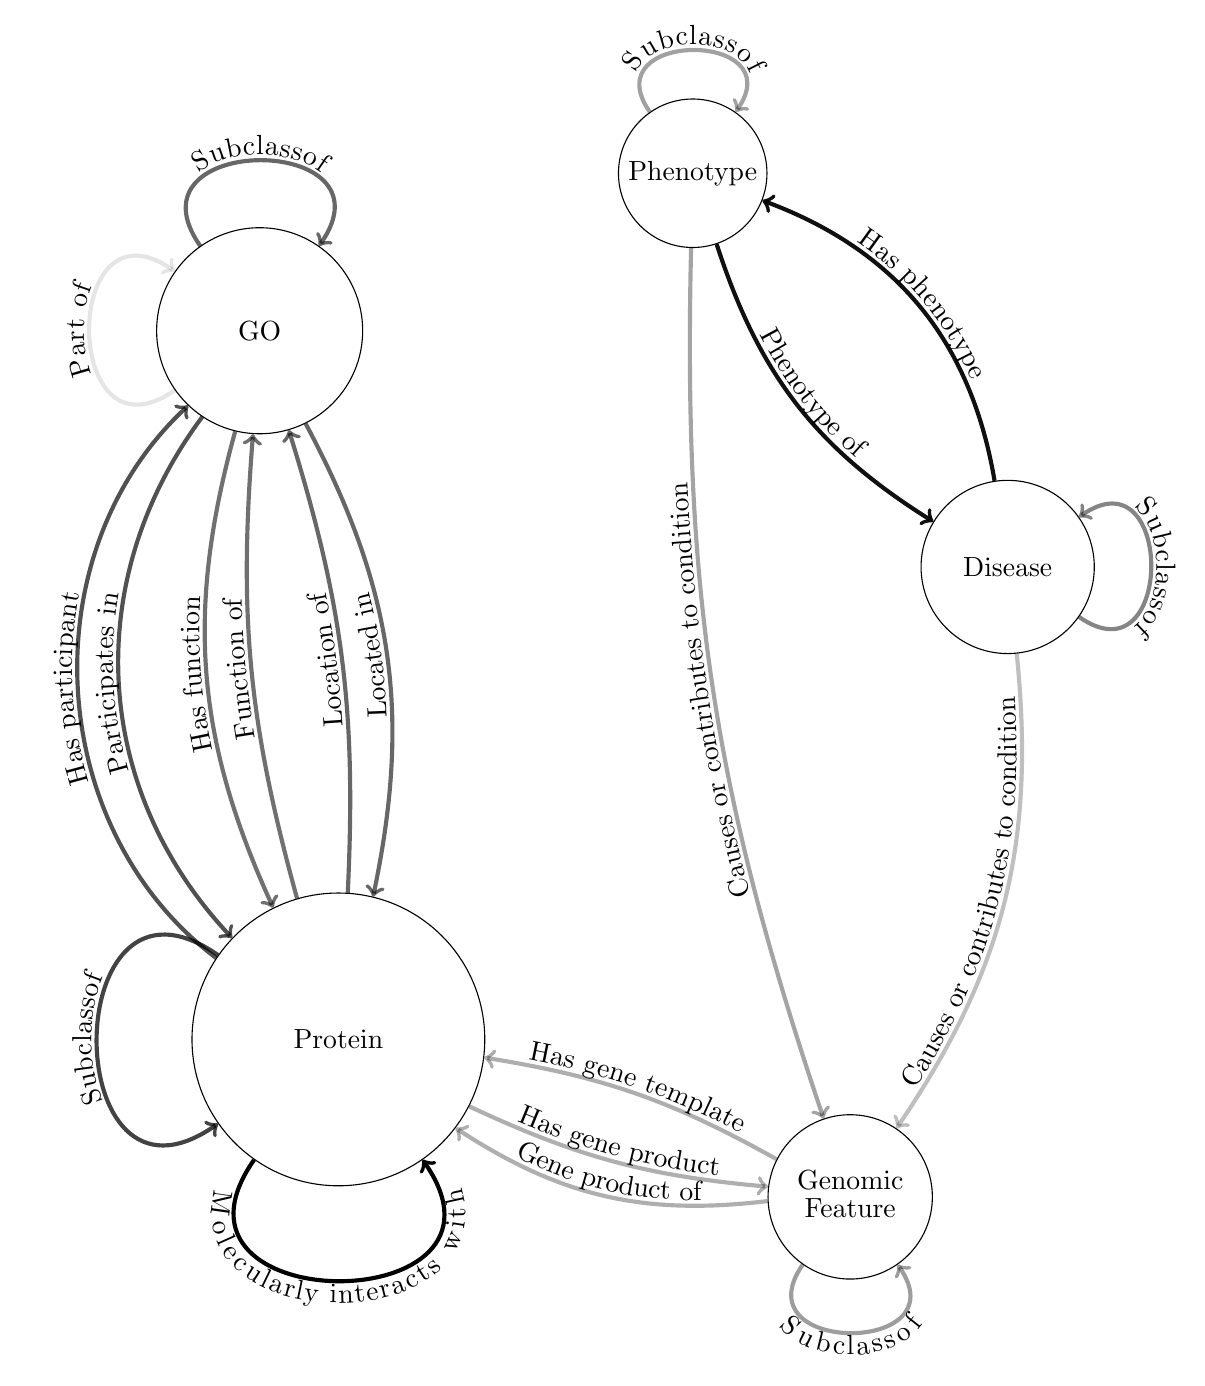
\begin{tikzpicture}
    \usetikzlibrary{decorations.text}

    \begin{scope}[xshift=1cm]
        % Nodes
        \node[circle, draw, fill=none, minimum size=3.718cm, inner sep=0pt] (Protein) at (-4,-3) {Protein};
        \node[circle, draw, fill=none, minimum size=2.617cm, inner sep=0pt] (GO) at (-5,6) {GO};
        \node[circle, draw, fill=none, minimum size=2.200cm, inner sep=0pt] (Disease) at (4.5,3) {Disease};
        \node[circle, draw, fill=none, minimum size=2.087cm, inner sep=0pt] (GenomicFeature) at (2.5,-5) {\begin{tabular}{c}Genomic\\[-0.5ex]Feature\end{tabular}};
        \node[circle, draw, fill=none, minimum size=1.886cm, inner sep=0pt] (Phenotype) at (0.5,8) {Phenotype};

        % Edges with curved labels
            \draw[->, line width=1.5pt, opacity=0.937927] (Disease) to[bend right=30] (Phenotype);
            \path[decorate, decoration={text along path, text align=center, raise=2pt, text={Has phenotype}}] (Phenotype) to[bend left=30] (Disease);

            \draw[->, line width=1.5pt, opacity=1.000000] (Protein) to[out=235, in=305, looseness=3] (Protein);
            \path[decorate, decoration={text along path, text align=center, raise=-8pt, text={Molecularly interacts with}}] (Protein) to[out=235, in=305, looseness=3](Protein);

            \draw[->, line width=1.5pt, opacity=0.478617] (Disease) to[out=-35, in=35, looseness=3] (Disease);
            \path[decorate, decoration={text along path, text align=center, raise=2pt, text={Subclassof}}] (Disease) to[out=35, in=-35, looseness=3] (Disease);

            \draw[->, line width=1.5pt, opacity=0.596164] (GO) to[out=125, in=55, looseness=3] (GO);
            \path[decorate, decoration={text along path, text align=center, raise=2pt, text={Subclassof}}] (GO) to[out=125, in=55, looseness=3] (GO);

            \draw[->, line width=1.5pt, opacity=0.383857] (GenomicFeature) to[out=235, in=305, looseness=3] (GenomicFeature);
            \path[decorate, decoration={text along path, text align=center, raise=-8pt, text={Subclassof}}] (GenomicFeature) to[out=235, in=305, looseness=3] (GenomicFeature);

            \draw[->, line width=1.5pt, opacity=0.367024] (Phenotype) to[out=125, in=55, looseness=3] (Phenotype);
            \path[decorate, decoration={text along path, text align=center, raise=2pt, text={Subclassof}}] (Phenotype) to[out=125, in=55, looseness=3] (Phenotype);

            \draw[->, line width=1.5pt, opacity=0.735558] (Protein) to[out=145, in=215, looseness=3] (Protein);
            \path[decorate, decoration={text along path, text align=center, raise=2pt, text={Subclassof}}] (Protein) to[out=215, in=145, looseness=3] (Protein);

            \draw[->, line width=1.5pt, opacity=0.561965] (Protein) to[bend left=10] (GO);
            \path[decorate, decoration={text along path, text align=center, raise=2pt, text={Function of}}] (Protein) to[bend left=10] (GO);


            \draw[->, line width=1.5pt, opacity=0.937927] (Phenotype) to[bend right=20] (Disease);
            \path[decorate, decoration={text along path, text align=center, raise=2pt, text={Phenotype of}}] (Phenotype) to[bend right=20] (Disease);

            \draw[->, line width=1.5pt, opacity=0.316749] (GenomicFeature) to[bend right=10] (Protein);
            \path[decorate, decoration={text along path, text align=center, raise=2pt, text={Has gene template}}] (Protein) to[bend left=10] (GenomicFeature);

            \draw[->, line width=1.5pt, opacity=0.561965] (GO) to[bend right=20] (Protein);
            \path[decorate, decoration={text along path, text align=center, raise=2pt, text={Has function}}] (Protein) to[bend left=20] (GO);

            \draw[->, line width=1.5pt, opacity=0.681528] (Protein) to[bend left=50] (GO);
            \path[decorate, decoration={text along path, text align=center, raise=2pt, text={Has participant}}] (Protein) to[bend left=50] (GO);

            \draw[->, line width=1.5pt, opacity=0.311908] (Protein) to[bend right=10] (GenomicFeature);
            \path[decorate, decoration={text along path, text align=center, raise=2pt, text={Has gene product}}] (Protein) to[bend right=10] (GenomicFeature);

           

            \draw[->, line width=1.5pt, opacity=0.595817] (Protein) to[bend right=10] (GO);
            \path[decorate, decoration={text along path, text align=center, raise=2pt, text={Location of}}] (Protein) to[bend right=10] (GO);

            \draw[->, line width=1.5pt, opacity=0.595822] (GO) to[bend left=20] (Protein);
            \path[decorate, decoration={text along path, text align=center, raise=2pt, text={Located in}}] (Protein) to[bend right=20] (GO);

            \draw[->, line width=1.5pt, opacity=0.681523] (GO) to[bend right=40] (Protein);
            \path[decorate, decoration={text along path, text align=center, raise=2pt, text={Participates in}}] (Protein) to[bend left=40] (GO);

            \draw[->, line width=1.5pt, opacity=0.250632] (Disease) to[bend left=20] (GenomicFeature);
            \path[decorate, decoration={text along path, text align=center, raise=2pt, text={Causes or contributes to condition}}] (GenomicFeature) to[bend right=20] (Disease);

            \draw[->, line width=1.5pt, opacity=0.356471] (Phenotype) to[bend right=10] (GenomicFeature);
            \path[decorate, decoration={text along path, text align=center, raise=2pt, text={Causes or contributes to condition}}] (GenomicFeature) to[bend left=10] (Phenotype);

            \draw[->, line width=1.5pt, opacity=0.311908] (GenomicFeature) to[bend left=20] (Protein);
            \path[decorate, decoration={text along path, text align=center, raise=2pt, text={Gene product of}}] (Protein) to[bend right=20] (GenomicFeature);

            \draw[->, line width=1.5pt, opacity=0.100000] (GO) to[out=215, in=145, looseness=3] (GO);
            \path[decorate, decoration={text along path, text align=center, raise=2pt, text={Part of}}] (GO) to[out=215, in=145, looseness=3] (GO);   \end{scope}
    \end{tikzpicture}

    \caption{A hypergraph representation of the underlying knowledge graph, having hypernodes representing the possibile node types and hyperedges for the most frequent edge predicates. The hypernodes' size and the hyperedges' opacity are logarithmic in the amount of node types and edge predicates respectively.}
    \label{fig:kg_hypergraph}
\end{figure}
The relations between the entities and their predicates derive from the annotations specified in the ontologies.

In terms of magnitude, the knowledge graph comprises a total of $2.34\cdot10^5$ heterogeneous nodes and $2.71\cdot10^7$ heterogeneous edges. The graph contains a total of six node types and 117 edge predicates. In \Cref{fig:kg_hypergraph}, we show the hypergraph representation of the knowledge graph obtained by aggregating the ontological data sources. To simplify the representation, we specified edge predicates with a minimum of $10^5$ occurrences across the entire knowledge graph. The number of nodes of each type is provided in \Cref{tab:nodetypes}, alongside the distribution of (the most frequent) edge predicates among the node types, as shown in \Cref{tab:edgedistrib}.
\begin{figure}
    \centering
        \begin{tikzpicture}
        [edge from parent fork down,
        sibling distance=40mm,
        every node/.style={anchor=west, align=center}]
        \small
        \node {disease } 
        [sibling distance=30mm]
        child {node {human disease}
            [sibling distance=35mm] 
            child {node {digestive system disorder}
                [sibling distance=32mm]
                child {node {intestinal disorder}
                    [sibling distance=37mm]
                    child {node {intestinal obstruction}
                        [sibling distance=15mm]
                        child {node {ileus}
                            [sibling distance=27mm]
                            child {node {meconium ileus}    
                                [sibling distance=65mm]                 
                                    child {node {\small \textbf{cystic fibrosis associated meconium ileus}}}                                        
                                    child {node {\dots}}                    }
                            child {node {\dots}}
                       }
                        child {node {\dots}}
                   }
                    child {node {\dots}}
               }
                child {node {\dots}}
           }
            child {node {\dots}}
       }
        child {node {perinatal disease}
            [sibling distance=0mm]
            child {node {\small \textbf{cystic fibrosis associated meconium ileus}}}
       }
        child {node {\dots}};
    \end{tikzpicture}
    \caption{A subtree composed of disease type nodes linked by \emph{subclassof} edges centered on the leaf disease \emph{cystic fibrosis associated meconium ileus} .}
    \label{fig:SubclassofTree}
\end{figure}
\paragraph{Abstract Graph Structure}\label{sec:abstractGraphStructure}
It is evident that the graph is connected, with certain edge predicates being mutually symmetric, e.g., \emph{has phenotype} and \emph{phenotype of}. For each of the node types, edges of the predicate \emph{Subclassof} denote hierarchical relationships between the entities. In \Cref{fig:SubclassofTree}, we illustrate a subtree representing one of these hierarchical components in the knowledge graph. For further examples, we suggest exploring the tree representations provided by the EMBL-EBI Ontology Lookup Service\footnote{Visit the EMBL-EBI Ontology Lookup Service at the link \url{https://www.ebi.ac.uk/ols4/}.}. One may visualize the knowledge graph as comprising ``vertical'' components, with one for each node type, akin to the example presented. In our discourse, we will refer to these subtrees as \term{hierarchical components}. These hierarchies are interconnected by ``horizontal'' links, which are indifferent to the hierarchical level of the nodes to which they pertain. This characteristic has led us to consider approaches based on hyperbolic geometry, as will be explored in \Cref{sec:hypPatientKG}.

\subsection{Patient data}
We have selected the patient data from the Phenopacket Store compiled by~\cite{Danis2025Phenopackets}, which is accessible at the dedicated repository~\cite{Robinson2024PhenopacketStore}. Our analyses are based on the most recent release to date, dated 19 January 2025 (version 0.1.24)\footnote{The phenopackets can be downloaded at \url{https://github.com/monarch-initiative/phenopacket-store/releases/download/0.1.24/all_phenopackets.zip}}, comprising 7799 cohorts.

The cohorts that represent individuals with Mendelian diseases adhere to the GA4GH Phenopacket Schema~\cite{jacobsen2022ga4ghPhenopacketSchema}\footnote{Comprehensive documentation can be found at \url{https://phenopacket-schema.readthedocs.io/en/latest/}}. The Phenopacket Schema represents an open standard for sharing disease and phenotype information, beneficial for both rare and common disease research. A Phenopacket integrates detailed phenotype descriptors with disease, patient, and genetic information, enabling the understanding of human diseases and biological phenomena.

For the patients collected in the Phenopacket Store, the following attributes are available:
\begin{itemize}
  \item patient code
  \item sex
  \item age at last encounter
  \item phenotypes, with optional specification of the year of onset
  \item diagnosed disease, with optional specification of the year of onset and genomic interpretations
  \item reference to the research article
\end{itemize}

We opted to focus on features that are consistently present in all cohorts or described with a similar level of detail. Consequently, we excluded the year of onset for individual phenotypes and the onset of the disease. Furthermore, noting that genomic interpretations are not always included, this aspect will be addressed through the links in the underlying knowledge graph described in the preceding section. We also removed the age of last encounter of the patient, as it is frequently unrelated to the diagnosed disease.

Given the inherent limitations of patient data regarding Mendelian diseases, we acknowledge that the dataset comprises a considerable number of diseases for which the number of cohorts is markedly low. To characterize the distribution of the Mendelian diseases available to us, we present in \Cref{fig:disease-histogram} a plot of occurrences for each disease in the Phenopacket Store, arranged in descending order.
\begin{figure}        
\centering
\begin{adjustbox}{margin=-1cm 0cm 0cm 0cm} % Left, Bottom, Right, Top margins

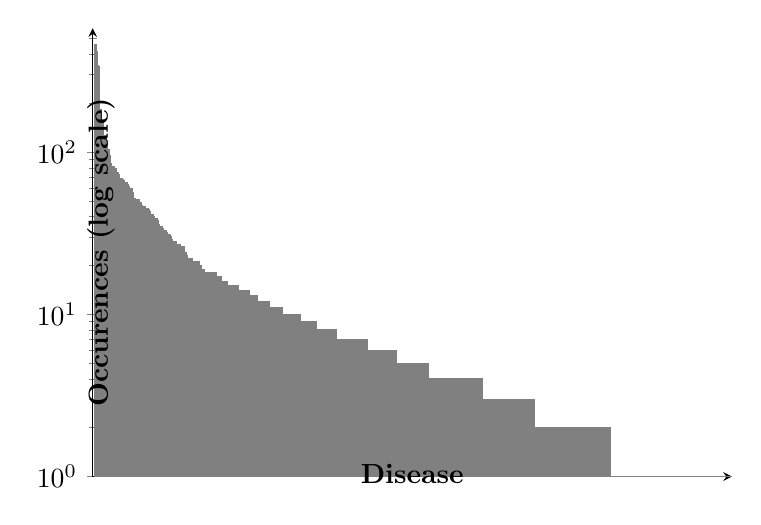
\begin{tikzpicture}
\begin{axis}[
    ybar,
    xmin=-2,
    ymin=-10,
    ymax=580,
    ymode=log, % Using logarithmic scale for y-axis
    log basis y=10,
    bar width=0.5pt,
    axis lines=left,
    width=0.8\textwidth,  % Scale to full text width
    height=0.6\textwidth, % Optional, for aspect ratio
    xlabel= {Disease},
    ylabel= {Occurences (log scale)},
    ylabel shift=-35pt, % Moves the y-label closer to the axis
    xlabel shift=-10pt, % Moves the x-label closer to the axis
    label style={font=\bfseries, fill=none},
    xtick=\empty,
    xticklabels=\empty,
    yticklabel style={fill=none}
    ]
\addplot+[
    fill=gray,
    draw=gray,
] coordinates {
    (0, 463)
 (1, 419)
 (2, 342)
 (3, 337)
 (4, 183)
 (5, 158)
 (6, 156)
 (7, 127)
 (8, 125)
 (9, 117)
 (10, 104)
 (11, 95)
 (12, 85)
 (13, 82)
 (14, 81)
 (15, 79)
 (16, 79)
 (17, 75)
 (18, 73)
 (19, 69)
 (20, 69)
 (21, 68)
 (22, 67)
 (23, 65)
 (24, 65)
 (25, 63)
 (26, 61)
 (27, 60)
 (28, 60)
 (29, 56)
 (30, 52)
 (31, 51)
 (32, 51)
 (33, 51)
 (34, 49)
 (35, 49)
 (36, 47)
 (37, 46)
 (38, 46)
 (39, 45)
 (40, 45)
 (41, 44)
 (42, 43)
 (43, 41)
 (44, 41)
 (45, 40)
 (46, 39)
 (47, 39)
 (48, 38)
 (49, 36)
 (50, 35)
 (51, 35)
 (52, 34)
 (53, 33)
 (54, 33)
 (55, 32)
 (56, 31)
 (57, 31)
 (58, 30)
 (59, 29)
 (60, 28)
 (61, 28)
 (62, 28)
 (63, 27)
 (64, 27)
 (65, 27)
 (66, 26)
 (67, 26)
 (68, 26)
 (69, 24)
 (70, 23)
 (71, 22)
 (72, 22)
 (73, 22)
 (74, 22)
 (75, 21)
 (76, 21)
 (77, 21)
 (78, 21)
 (79, 21)
 (80, 20)
 (81, 20)
 (82, 19)
 (83, 19)
 (84, 18)
 (85, 18)
 (86, 18)
 (87, 18)
 (88, 18)
 (89, 18)
 (90, 18)
 (91, 18)
 (92, 18)
 (93, 17)
 (94, 17)
 (95, 17)
 (96, 17)
 (97, 16)
 (98, 16)
 (99, 16)
 (100, 16)
 (101, 16)
 (102, 15)
 (103, 15)
 (104, 15)
 (105, 15)
 (106, 15)
 (107, 15)
 (108, 15)
 (109, 15)
 (110, 14)
 (111, 14)
 (112, 14)
 (113, 14)
 (114, 14)
 (115, 14)
 (116, 14)
 (117, 14)
 (118, 14)
 (119, 13)
 (120, 13)
 (121, 13)
 (122, 13)
 (123, 13)
 (124, 13)
 (125, 12)
 (126, 12)
 (127, 12)
 (128, 12)
 (129, 12)
 (130, 12)
 (131, 12)
 (132, 12)
 (133, 12)
 (134, 11)
 (135, 11)
 (136, 11)
 (137, 11)
 (138, 11)
 (139, 11)
 (140, 11)
 (141, 11)
 (142, 11)
 (143, 11)
 (144, 10)
 (145, 10)
 (146, 10)
 (147, 10)
 (148, 10)
 (149, 10)
 (150, 10)
 (151, 10)
 (152, 10)
 (153, 10)
 (154, 10)
 (155, 10)
 (156, 10)
 (157, 10)
 (158, 9)
 (159, 9)
 (160, 9)
 (161, 9)
 (162, 9)
 (163, 9)
 (164, 9)
 (165, 9)
 (166, 9)
 (167, 9)
 (168, 9)
 (169, 9)
 (170, 8)
 (171, 8)
 (172, 8)
 (173, 8)
 (174, 8)
 (175, 8)
 (176, 8)
 (177, 8)
 (178, 8)
 (179, 8)
 (180, 8)
 (181, 8)
 (182, 8)
 (183, 8)
 (184, 8)
 (185, 7)
 (186, 7)
 (187, 7)
 (188, 7)
 (189, 7)
 (190, 7)
 (191, 7)
 (192, 7)
 (193, 7)
 (194, 7)
 (195, 7)
 (196, 7)
 (197, 7)
 (198, 7)
 (199, 7)
 (200, 7)
 (201, 7)
 (202, 7)
 (203, 7)
 (204, 7)
 (205, 7)
 (206, 7)
 (207, 7)
 (208, 7)
 (209, 6)
 (210, 6)
 (211, 6)
 (212, 6)
 (213, 6)
 (214, 6)
 (215, 6)
 (216, 6)
 (217, 6)
 (218, 6)
 (219, 6)
 (220, 6)
 (221, 6)
 (222, 6)
 (223, 6)
 (224, 6)
 (225, 6)
 (226, 6)
 (227, 6)
 (228, 6)
 (229, 6)
 (230, 6)
 (231, 5)
 (232, 5)
 (233, 5)
 (234, 5)
 (235, 5)
 (236, 5)
 (237, 5)
 (238, 5)
 (239, 5)
 (240, 5)
 (241, 5)
 (242, 5)
 (243, 5)
 (244, 5)
 (245, 5)
 (246, 5)
 (247, 5)
 (248, 5)
 (249, 5)
 (250, 5)
 (251, 5)
 (252, 5)
 (253, 5)
 (254, 5)
 (255, 5)
 (256, 4)
 (257, 4)
 (258, 4)
 (259, 4)
 (260, 4)
 (261, 4)
 (262, 4)
 (263, 4)
 (264, 4)
 (265, 4)
 (266, 4)
 (267, 4)
 (268, 4)
 (269, 4)
 (270, 4)
 (271, 4)
 (272, 4)
 (273, 4)
 (274, 4)
 (275, 4)
 (276, 4)
 (277, 4)
 (278, 4)
 (279, 4)
 (280, 4)
 (281, 4)
 (282, 4)
 (283, 4)
 (284, 4)
 (285, 4)
 (286, 4)
 (287, 4)
 (288, 4)
 (289, 4)
 (290, 4)
 (291, 4)
 (292, 4)
 (293, 4)
 (294, 4)
 (295, 4)
 (296, 4)
 (297, 3)
 (298, 3)
 (299, 3)
 (300, 3)
 (301, 3)
 (302, 3)
 (303, 3)
 (304, 3)
 (305, 3)
 (306, 3)
 (307, 3)
 (308, 3)
 (309, 3)
 (310, 3)
 (311, 3)
 (312, 3)
 (313, 3)
 (314, 3)
 (315, 3)
 (316, 3)
 (317, 3)
 (318, 3)
 (319, 3)
 (320, 3)
 (321, 3)
 (322, 3)
 (323, 3)
 (324, 3)
 (325, 3)
 (326, 3)
 (327, 3)
 (328, 3)
 (329, 3)
 (330, 3)
 (331, 3)
 (332, 3)
 (333, 3)
 (334, 3)
 (335, 3)
 (336, 3)
 (337, 2)
 (338, 2)
 (339, 2)
 (340, 2)
 (341, 2)
 (342, 2)
 (343, 2)
 (344, 2)
 (345, 2)
 (346, 2)
 (347, 2)
 (348, 2)
 (349, 2)
 (350, 2)
 (351, 2)
 (352, 2)
 (353, 2)
 (354, 2)
 (355, 2)
 (356, 2)
 (357, 2)
 (358, 2)
 (359, 2)
 (360, 2)
 (361, 2)
 (362, 2)
 (363, 2)
 (364, 2)
 (365, 2)
 (366, 2)
 (367, 2)
 (368, 2)
 (369, 2)
 (370, 2)
 (371, 2)
 (372, 2)
 (373, 2)
 (374, 2)
 (375, 2)
 (376, 2)
 (377, 2)
 (378, 2)
 (379, 2)
 (380, 2)
 (381, 2)
 (382, 2)
 (383, 2)
 (384, 2)
 (385, 2)
 (386, 2)
 (387, 2)
 (388, 2)
 (389, 2)
 (390, 2)
 (391, 2)
 (392, 2)
 (393, 2)
 (394, 2)
 (395, 1)
 (396, 1)
 (397, 1)
 (398, 1)
 (399, 1)
 (400, 1)
 (401, 1)
 (402, 1)
 (403, 1)
 (404, 1)
 (405, 1)
 (406, 1)
 (407, 1)
 (408, 1)
 (409, 1)
 (410, 1)
 (411, 1)
 (412, 1)
 (413, 1)
 (414, 1)
 (415, 1)
 (416, 1)
 (417, 1)
 (418, 1)
 (419, 1)
 (420, 1)
 (421, 1)
 (422, 1)
 (423, 1)
 (424, 1)
 (425, 1)
 (426, 1)
 (427, 1)
 (428, 1)
 (429, 1)
 (430, 1)
 (431, 1)
 (432, 1)
 (433, 1)
 (434, 1)
 (435, 1)
 (436, 1)
 (437, 1)
 (438, 1)
 (439, 1)
 (440, 1)
 (441, 1)
 (442, 1)
 (443, 1)
 (444, 1)
 (445, 1)
 (446, 1)
 (447, 1)
 (448, 1)
 (449, 1)
 (450, 1)
 (451, 1)
 (452, 1)
 (453, 1)
 (454, 1)
 (455, 1)
 (456, 1)
 (457, 1)
 (458, 1)
 (459, 1)
 (460, 1)
 (461, 1)
 (462, 1)
 (463, 1)
 (464, 1)
 (465, 1)
 (466, 1)
 (467, 1)
 (468, 1)
 (469, 1)
 (470, 1)
 (471, 1)
 (472, 1)
 (473, 1)
 (474, 1)
 (475, 1)
 (476, 1)
 (477, 1)
 (478, 1)
 (479, 1)
 (480, 1)
 (481, 1)
 (482, 1)
 (483, 1)
 (484, 1)
 (485, 1)
 (486, 1)
 (487, 1)
 (488, 1)



};
\end{axis}
\end{tikzpicture}
\end{adjustbox}
\caption{Bar plot of Mendelian disease occurrence distribution in the Phenopacket Store.}
\label{fig:disease-histogram}
\end{figure}


\subsection{Data integration}
The patient data has been integrated with the underlying knowledge graph by adding nodes of type \emph{Person} and \emph{Article}. Specifically, the \emph{Person} nodes encompass the actual patients, alongside two nodes representing male and female sexes, respectively. For standardization purposes, the \emph{Male} and \emph{Female} nodes are identified using the following IRIs: \texttt{$\langle$http://purl.obolibrary.org/obo/NCIT\_C16576$\rangle$} and \texttt{$\langle$http://purl.obolibrary.org/obo/NCIT\_C20197$\rangle$}. Each article is refered to by \\ \texttt{$\langle$https://pubmed.ncbi.nlm.nih.gov/{article\_id}$\rangle$}. The nodes pertaining to patients extend the \emph{Article} identifiers by appending the patient code, resulting in a string of the form \\ \texttt{$\langle$https://pubmed.ncbi.nlm.nih.gov/{article\_id}?{patient\_code}$\rangle$}. 

We clarify the integration of the Phenopacket data with the underlying knowledge graph in \Cref{fig:patient_kg_hypergraph}, which specifies how the additional nodes have been interconnected with one another and with the existing \emph{Phenotype} and \emph{Disease} nodes. Henceforth, we will refer to the integrated knowledge graph as \emph{PatientKG}.
\begin{figure}
    \centering
    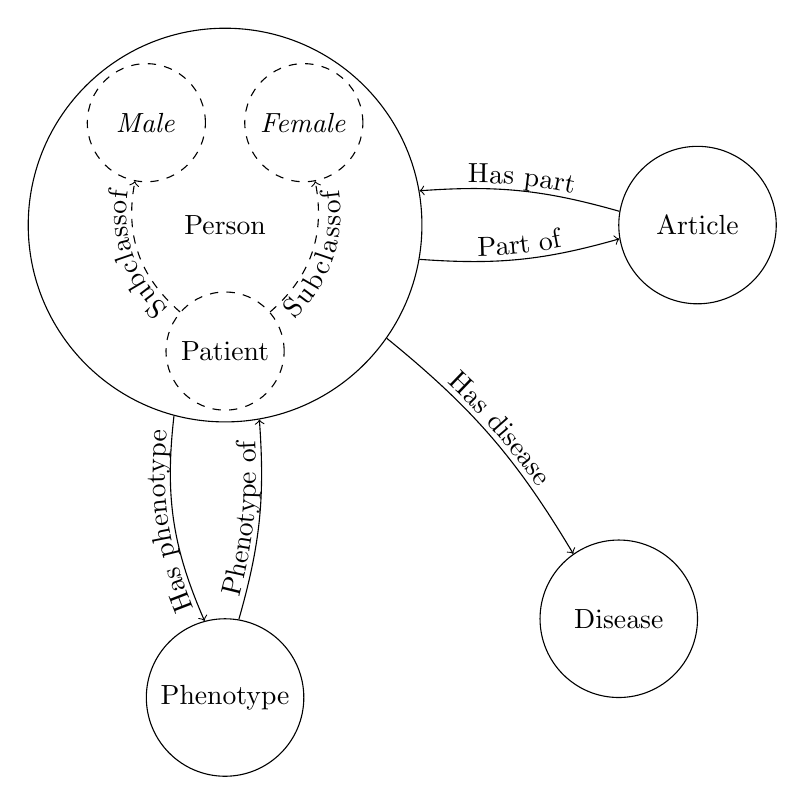
\begin{tikzpicture}
        % Nodes
        \node[circle, draw, fill=none, minimum size=2cm, inner sep=0pt] (Disease) at (1,4) {Disease};
        \node[circle, draw, fill=none, minimum size=2cm, inner sep=0pt] (Phenotype) at (-4,3) {Phenotype};
        \node[circle, draw, fill=none, minimum size=2cm, inner sep=0pt] (Article) at (2,9) {Article};
        \node[circle, draw, fill=none, minimum size=5cm, inner sep=0pt] (Person) at (-4,9) {Person};
        \node[circle, draw, dashed,  fill=none, minimum size=1.5cm, inner sep=0pt] (Male) at (-5,10.3) {\textit{Male}};
        \node[circle, draw, dashed, fill=none, minimum size=1.5cm, inner sep=0pt] (Female) at (-3,10.3) {\textit{Female}};
        \node[circle, draw, dashed, fill=none, minimum size=1.5cm, inner sep=0pt] (Patient) at (-4,7.4) {Patient};

        % Edges with curved labels
            \draw[->] (Person) to[bend right=10] (Article);
            \path[decorate, decoration={text along path, text align=center, raise=2pt, text={Part of}}] (Person) to[bend right=10] (Article);

            \draw[->] (Article) to[bend right=10] (Person);
            \path[decorate, decoration={text along path, text align=center, raise=2pt, text={Has part}}] (Person) to[bend left=10] (Article);

            \draw[dashed, ->] (Patient) to[bend left=30] (Male);
            \path[decorate, decoration={text along path, text align=center, raise=2pt, text={Subclassof}}] (Patient) to[bend left=30] (Male);
            \draw[dashed, ->] (Patient) to[bend right=30] (Female);
            \path[decorate, decoration={text along path, text align=center, raise=-8pt, text={Subclassof}}] (Patient) to[bend right=30] (Female);

            \draw[->] (Person) to[bend left=10] (Disease);
            \path[decorate, decoration={text along path, text align=center, raise=2pt, text={Has disease}}] (Person) to[bend left=10] (Disease);

            \draw[->] (Person) to[bend right=15] (Phenotype);
            \path[decorate, decoration={text along path, text align=center, raise=2pt, text={Has phenotype}}] (Phenotype) to[bend left=15] (Person);
            \draw[->] (Phenotype) to[bend right=10] (Person);
            \path[decorate, decoration={text along path, text align=center, raise=2pt, text={Phenotype of}}] (Phenotype) to[bend right=10] (Person);
    \end{tikzpicture}

    \caption{The hypergraph representing the node types and edge predicates added during the integration of the underlying knowledge graph and patient data. The nodes contained in the Person hypernode and the relative hyperedges are merely a semantic schematization of the data. In particular Male and Female correspond to single nodes in the knowledge graph.}
    \label{fig:patient_kg_hypergraph}
\end{figure}

\section{Link prediction for differential diagnosis}\label{sec:linkPredictionDiffDiagnosis}
In this section, we describe how we have employed PatientKG to address the challenge of differential diagnosis. We first adapt the problem to the PatientKG at our disposal.

\subsection{Experiment Setup}
Utilizing PatientKG, the problem of differential diagnosis is reframed as the link prediction task involving edges of type \emph{Has disease} connecting the \emph{Person} nodes representing patients to the corresponding \emph{Disease} node. Considering the techniques evaluated in \Cref{grl}, we have chosen an inductive approach, specifically Graph Neural Networks (GNNs), to enable the model to generalize to previously unseen patients. In particular, we have selected the HGCN model, according to the reasoning discussed in \Cref{sec:hypPatientKG}.

To train the model for link prediction and evaluate its performance, the edges in PatientKG were partitioned into two sets: a test set composed of randomly selected \emph{Has disease} edges and a training set comprising the remaining \emph{Has disease} edges and all other edges in PatientKG. To regulate the learning process through early stopping, we also have extracted a validation set.

Given the limited availability of annotated disease diagnoses, we opted not to include \emph{Has disease} edges within the validation set utilized to monitor the learning process. The distribution of cohorts by disease, illustrated in \Cref{fig:disease-histogram}, indicates that approximately half of the diseases represented in the Phenopacket Store have fewer than 10 cohorts, and roughly one-third have at most 5 occurrences.

Since the test edges are derived from the relations provided by the Phenopacket Store, the model trained on the training set will be evaluated on differential diagnoses exclusively among Mendelian diseases. This approach is logical as Mendelian diseases are often explored after all alternative common diagnoses have been ruled out. Preliminary experiments conducted using this data split revealed indications of potential overfitting. Since the articles typically pertain to specific diseases, the edges connecting patients to their corresponding articles of origin create a shortcut for inferring the patients' diseases. To prevent data leakage, we excluded all \emph{Has part} and \emph{Part of} edges linking the \emph{Person} nodes to the \emph{Article} nodes.

\subsection{Why hyperbolic graph representation learning?}\label{sec:hypPatientKG}
Prior to delving into the run experiments, we would like to account for the selection of hyperbolic graph representation learning techniques, specifically HGCN. As discussed in \Cref{sec:hyperbolicAndTrees}, hyperbolic geometry is particularly suited to represent hierarchical structures, such as those nested within PatientKG (refer to \Cref{sec:abstractGraphStructure}). To empirically verify this, we embedded each hierarchical component into hyperbolic space. To emphasize the positioning of each node within the hierarchy, we have considered the transitive closure of each subtree. The transitive closure of a directed graph is derived by adding an edge between every pair of nodes that are connected by a directed path. For instance, \Cref{fig:diseasePoincare} depicts the embedded \emph{Disease} nodes arranged within a Poincaré ball. One notices that nodes with a more extensive neighbourhood, i.e. nodes situated higher in the ontological hierarchy, are positioned closer to the centre of the ball. This representation can be interpreted as a real-world instance of the structure schematized in \Cref{fig:radialTree}, in accordance with the considerations articulated in \Cref{sec:expGrowth}. 
\begin{figure}
    \centering
    \begin{subfigure}[b]{0.6\textwidth}
        \centering
        \includegraphics[width=\textwidth]{figs/figDiseasePoincare.png}
    \end{subfigure}
    \begin{subfigure}[b]{0.1\textwidth}
        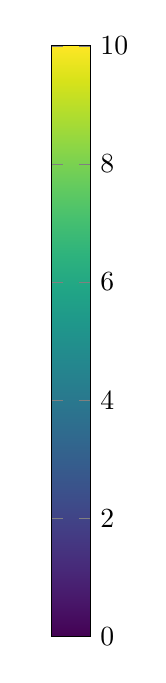
\begin{tikzpicture}
            \begin{axis}[
                hide axis,
                scale only axis,
                height=7.5cm,
                colorbar,
                colormap name=viridis,
                point meta min=0,
                point meta max=10,
                colorbar style={
                    height=7.5cm,
                    width=0.5cm,
                    ytick={0,2,...,10},
                    ticklabel style={fill=none, draw=none},
                    }      
                ]
                \addplot [draw=none, fill=none] coordinates {(0,0)};
            \end{axis}
        \end{tikzpicture}
    \end{subfigure}
    \label{fig:diseasePoincare}
    \caption{Shallow hyperbolic embeddings in the Poincaré disk of the \emph{Disease} hierarchical component. The color scale refers to the size of the neighbourhood of each node, in logarithmic scale.}

\end{figure}

Although the shallow embedding has yielded favorable results, we opted for an inductive graph representation technique, as touched on in the previous section. To ensure that the HGCN model would capture the hierarchical components within PatientKG, we assessed the model's performance exclusively on these subgraphs. In comparison, we conducted the same experiments using two representatives of advanced Euclidean GNN models, namely GCN (\Cref{sec:GCN}) and GAT (\Cref{sec:neighbourhoodAttention}). The hyperparameters employed in our experiments are detailed in Table~\ref{tab:hyperparams}; the number of attention heads is overlooked by the GCN model. For HGCN learning, the parameters for the Fermi-Dirac decoder are set to \texttt{r}=2 and \texttt{t}=1 (refer to \Cref{sec:linkPredictionHGCN}). These values were established based on hyperparameters recommended in the code repository provided by Hazy Research, which encompasses implementations of HGCN and other Euclidean and hyperbolic GNN models\footnote{We have utilized the implementations offered by the Hazy Research group at \url{https://github.com/HazyResearch/hgcn}. In particular, we have relied on their code for the shallow Poincaré ball embeddings, GCN, GAT models, and, of course, HGCN.}. 
\begin{table}
    \centering
    \caption{Hyperparameters used for training GCN, GAT and HGCN.}
    \label{tab:hyperparams}
    \begin{tabular}{rl}
        \toprule
        \textbf{Hyperparameter} & \textbf{Value} \\
        \midrule
        \texttt{Number of layers} & 2 \\
        \texttt{Number of heads} &  4 \\
        \texttt{Weight decay} & 0.001 \\
        \texttt{Learning rate} & 0.01 \\
        \texttt{LR reduce frequency} & 5000 \\
        \texttt{Dropout} & 0.1 \\
        \texttt{Optimizer} & Adam \\
        \texttt{Momentum} & 0.999 \\
        \texttt{Gamma} & 0.5 \\
        \texttt{Activation function} & ReLU \\
        \texttt{Early stopping patience} & 200 \\
        \bottomrule
    \end{tabular}
\end{table}


In \Cref{tab:tabHypPerf}, we display the performance of the three models resulting from a random split of the edges into training, validation, and test sets, with validation and test sets containing 10\% of the edges each. We conducted a series of experiments while varying the desired embedding size. The evaluation of the predictions is expressed as the sum of the cross-entropy losses of positive and negative predictions, as well as the ROC\_AUC and average precision scores. As anticipated, performance improves upon increasing length of the hidden representation of the nodes. The results distinctly illustrate that HGCN surpasses Euclidean GNN models. The sole exception is observed within the \emph{Genomic feature} hierarchical component, where GCN and GAT yield slightly superior performance compared to HGCN at larger embedding sizes. In such instances, the loss remains elevated, suggesting that the models may be making incorrect predictions confidently. These tests confirm our confidence in employing HGCN for the link prediction task within PatientKG.
\begin{table}
    \centering
    \begin{subtable}[t]{\textwidth}
        \centering
        \begin{tabular}{l|ccc|ccc|ccc}        
            \toprule
            \multirow{2}{*}{\textbf{size}} & \multicolumn{3}{c}{\textit{Loss}} & \multicolumn{3}{c}{\textit{ROC\_AUC}} & \multicolumn{3}{c}{\textit{AP score}} \\
            & \textbf{GCN} & \textbf{GAT} & \textbf{HGCN} & \textbf{GCN} & \textbf{GAT} & \textbf{HGCN} & \textbf{GCN} & \textbf{GAT} & \textbf{HGCN} \\
            \midrule
                4 & 2.2522 & 2.2536 & \underline{1.2305} & 0.6289 & 0.5488 & \underline{0.9118} & 0.5913 & 0.5102 & \underline{0.9106} \\  
                8 & 2.2538 & 2.2523 & \underline{0.9730} & 0.6764 & 0.5836 & \underline{0.9442} & 0.6440 & 0.5744 & \underline{0.9584} \\
                16 & 2.2538 & - & \underline{0.8388} & 0.7117 & - & \underline{0.9479} & 0.7067 & - & \underline{0.9615} \\
                32 & 2.2538 & - & \underline{0.8666} & 0.7646 & - & \underline{0.9527} & 0.7444 & - & \underline{0.9647} \\
                64 & 2.2538 & - & \underline{0.8539} & 0.7901 & - & \underline{0.9484} & 0.7612 & - & \underline{0.9637} \\
                100 & 2.2537 & 2.2451 & \underline{0.6406} & 0.8012 & 0.7107 & \underline{0.9573} & 0.7973 & 0.7415 & \underline{0.9604} \\
            \bottomrule
        \end{tabular}
        \caption{Node type \textit{Disease}}
    \end{subtable}
    
    \vspace{1em}
    
    \begin{subtable}[t]{\textwidth}
        \centering
        \begin{tabular}{l|ccc|ccc|ccc}      
            \toprule
            \multirow{2}{*}{\textbf{size}} & \multicolumn{3}{c}{\textit{Loss}} & \multicolumn{3}{c}{\textit{ROC\_AUC}} & \multicolumn{3}{c}{\textit{AP score}} \\
            & \textbf{GCN} & \textbf{GAT} & \textbf{HGCN} & \textbf{GCN} & \textbf{GAT} & \textbf{HGCN} & \textbf{GCN} & \textbf{GAT} & \textbf{HGCN} \\
            4 & 2.2539 & 2.2532 & \underline{2.3959} & \underline{0.7094} & 0.5958 & 0.7459 & \underline{0.6371} & 0.5268 & 0.6906 \\
            8 & 2.2538 & 2.2521 & \underline{1.3602} & 0.7353 & 0.5918 & \underline{0.8838} & 0.6796 & 0.5350 & \underline{0.8751} \\
            16 & 2.2538 & 2.2517 & \underline{1.0282} & 0.7770 & 0.6673 & \underline{0.9193} & 0.7415 & 0.6436 & \underline{0.9119} \\
            32 & 2.2538 & 2.2507 & \underline{1.0209} & 0.8628 & 0.7112 & \underline{0.9317} & 0.8249 & 0.7301 & \underline{0.9307} \\
            64 & 2.2533 & 2.2492 & \underline{1.3956} & \underline{0.9333} & 0.7374 & 0.8922 & \underline{0.9256} & 0.7765 & 0.9109 \\
            100 & 2.2538 & 2.2433 & \underline{1.0364} & \underline{0.9683} & 0.7604 & 0.9232 & \underline{0.9539} & 0.8028 & 0.9159 \\
            \bottomrule
        \end{tabular}
        \caption{Node type \textit{Genomic feature}}
        \end{subtable}
    
    \vspace{1em}
    
    \begin{subtable}[t]{\textwidth}
        \centering
        \begin{tabular}{l|ccc|ccc|ccc}   
             \toprule
                \multirow{2}{*}{\textbf{size}} & \multicolumn{3}{c}{\textit{Loss}} & \multicolumn{3}{c}{\textit{ROC\_AUC}} & \multicolumn{3}{c}{\textit{AP score}} \\
                & \textbf{GCN} & \textbf{GAT} & \textbf{HGCN} & \textbf{GCN} & \textbf{GAT} & \textbf{HGCN} & \textbf{GCN} & \textbf{GAT} & \textbf{HGCN} \\
                \midrule
                4 & 2.2538 & 2.2538 & \underline{0.8984} & 0.6441 & 0.6087 & \underline{0.7923} & 0.6152 & 0.5869 & \underline{0.8179} \\
                8 & 2.2538 & 2.2537 & \underline{0.7069} & 0.6627 & 0.6207 & \underline{0.8354} & 0.6513 & 0.6160 & \underline{0.8791} \\
                16 & 2.2538 & 2.2532 & \underline{0.6602} & 0.6992 & 0.6697 & \underline{0.8609} & 0.7059 & 0.6861 & \underline{0.8883} \\
                32 & 2.2538 & 2.2521 & \underline{0.6035} & 0.7403 & 0.6832 & \underline{0.8773} & 0.7265 & 0.7106 & \underline{0.9001} \\
                64 & 2.2535 & 2.2517 & \underline{0.5554} & 0.7569 & 0.7123 & \underline{0.9479} & 0.7598 & 0.7392 & \underline{0.9153} \\
                100 & 2.2534 & 2.2492 & \underline{0.5618} & 0.7742 & 0.7044 & \underline{0.9692} & 0.7749 & 0.7373 & \underline{0.9140} \\
                \bottomrule
        \end{tabular}
        \caption{Node type \textit{GO}}
    \end{subtable}
    
    \vspace{1em}
    
    \begin{subtable}[t]{\textwidth}
        \centering
        \begin{tabular}{l|ccc|ccc|ccc}   
        \toprule
            \multirow{2}{*}{\textbf{size}} & \multicolumn{3}{c}{\textit{Loss}} & \multicolumn{3}{c}{\textit{ROC\_AUC}} & \multicolumn{3}{c}{\textit{AP score}} \\
            & \textbf{GCN} & \textbf{GAT} & \textbf{HGCN} & \textbf{GCN} & \textbf{GAT} & \textbf{HGCN} & \textbf{GCN} & \textbf{GAT} & \textbf{HGCN} \\
            \midrule
            4 & 2.2539 & - & \underline{1.4855} & 0.6289 & - & \underline{0.9240} & 0.5947 & - & \underline{0.9460} \\
            8 & 2.2538 & - & \underline{1.3125} & 0.6501 & - & \underline{0.9334} & 0.6284 & - & \underline{0.9572} \\
            16 & 2.2538 & - & \underline{1.1390} & 0.6848 & - & \underline{0.9359} & 0.6728 & - & \underline{0.9594} \\
            32 & 2.2538 & - & \underline{0.9025} & 0.7036 & - & \underline{0.9382} & 0.7017 & - & \underline{0.9610} \\
            64 & 2.2538 & - & \underline{0.6700} & 0.7276 & - & \underline{0.9452} & 0.7119 & - & \underline{0.9633} \\
            100 & 2.2538 & 2.2389 & \underline{0.6079} & 0.7567 & 0.6555 & \underline{0.9573} & 0.7318 & 0.6771 & \underline{0.9688} \\
            \bottomrule
        \end{tabular}
        \caption{Node type \textit{Phenotype}}
    \end{subtable}
    \label{tab:tabHypPerf}
    \caption{Performance of models HCGN, GAT and GCN on hierarchical components in PatientKG across different node types}
\end{table}


We are aware of more advanced techniques than HGCN that are tailored to knowledge graph applications. In particular, we highlight the \textsc{Att\_H} model~\cite{chami2020lowDimensionalHyperbolicKnowledgeGraphEmbeddings}, proposed by the authors of HGCN. Their rationale is that existing hyperbolic embedding methods do not adequately account for the logical patterns present in knowledge graphs, which we have referred to as "horizontal" links. Consequently, they introduce a class of hyperbolic KG embedding models that simultaneously capture hierarchical and logical patterns by combining hyperbolic reflections and rotations with attention. We have chosen to stick with a model like HGCN that emphasizes the hierarchical components, as we were interested in evaluating whether this approach would be sufficient to address the challenges of differential diagnosis. We leave the exploration of more advanced hyperbolic models for future work.
